\documentclass[11pt]{article}

\usepackage[a4paper,margin=1in]{geometry}
\usepackage[T1]{fontenc}
\usepackage[utf8]{inputenc}
\usepackage{lmodern}
\usepackage{microtype}
\usepackage{xcolor}
\usepackage{amsmath,amssymb,amsthm,mathtools}
\usepackage{bm}
\usepackage{array,booktabs,multirow}
\usepackage{enumitem}
\usepackage{tikz}
\usetikzlibrary{arrows.meta,positioning,calc,fit}
\usepackage[most]{tcolorbox}
\usepackage{hyperref}
\usepackage{fancyhdr}
\usepackage{titlesec}
\usepackage{setspace}

\hypersetup{
  colorlinks=true,
  linkcolor=blue!50!black,
  urlcolor=blue!50!black,
  citecolor=blue!50!black,
  pdftitle={Coding Theory: Linear Codes and their Dual - Lecture Notes}
}

\definecolor{accent}{RGB}{38,84,124}
\definecolor{softaccent}{RGB}{232,240,248}
\definecolor{softgray}{RGB}{245,246,248}
\definecolor{rulegray}{RGB}{214,219,224}

\titleformat{\section}{\large\bfseries\color{accent}}{\thesection.}{0.6em}{}
\titleformat{\subsection}{\normalsize\bfseries\color{accent}}{\thesubsection.}{0.6em}{}
\titleformat{\subsubsection}{\normalsize\bfseries}{\thesubsubsection.}{0.6em}{}

\setlength{\parindent}{0pt}
\setlength{\parskip}{0.55em}
\setstretch{1.08}

\pagestyle{fancy}
\fancyhf{}
\fancyhead[L]{\textit{Coding Theory Lecture Notes}}
\fancyhead[R]{\textit{Linear Codes and their Dual}}
\fancyfoot[C]{\thepage}
\renewcommand{\headrulewidth}{0.4pt}
\renewcommand{\footrulewidth}{0pt}

\newtheorem{proposition}{Proposition}[section]
\newtheorem{theorem}[proposition]{Theorem}
\newtheorem{corollary}[proposition]{Corollary}
\theoremstyle{definition}
\newtheorem{definition}[proposition]{Definition}
\newtheorem{example}[proposition]{Example}
\newtheorem{exercise}[proposition]{Exercise}
\theoremstyle{remark}
\newtheorem*{remark}{Remark}

\newcommand{\F}{\mathbb{F}}
\newcommand{\code}{\mathcal{C}}
\newcommand{\dual}[1]{#1^{\perp}}
\newcommand{\vect}[1]{\bm{#1}}

\begin{document}

\begin{titlepage}
\centering
\vspace*{2cm}

{\color{accent}\rule{0.82\textwidth}{1.2pt}}\par
\vspace{0.8cm}
{
  \Huge\bfseries Coding Theory\\[0.35em]
  \LARGE Linear Codes and their Dual
}\par
\vspace{0.8cm}
{\color{accent}\rule{0.82\textwidth}{1.2pt}}\par
\vspace{1.2cm}

\begin{tcolorbox}[
  width=0.86\textwidth,
  colback=softaccent,
  colframe=accent!65,
  boxrule=0.8pt,
  arc=2mm,
  left=8pt,right=8pt,top=8pt,bottom=8pt
]
\large
These notes reorganize the slide deck into a continuous lecture-note format. The main goals are:
\begin{itemize}[leftmargin=1.4em,itemsep=0.35em,topsep=0.35em]
    \item to review generator and parity-check descriptions of linear codes,
    \item to define the dual code in two equivalent ways,
    \item to study the Hamming code, repetition code, single parity-check code, and tetracode,
    \item to explain self-orthogonal and self-dual codes through concrete matrix calculations.
\end{itemize}
\end{tcolorbox}

\vfill
{
ormalsize Prepared from the lecture slides \emph{Coding Theory: Linear Codes and their Dual}.}

\end{titlepage}

\tableofcontents
\vspace{0.8em}

\begin{tcolorbox}[
  colback=softgray,
  colframe=rulegray,
  boxrule=0.6pt,
  arc=1.5mm,
  left=8pt,right=8pt,top=6pt,bottom=6pt,
  title=Notation,
  coltitle=black,
  fonttitle=\bfseries
]
Throughout, $\F_q$ denotes a finite field with $q$ elements. A linear $(n,k)$ code over $\F_q$ is a $k$-dimensional subspace of $\F_q^n$. We write vectors as row vectors unless explicitly transposed.
\end{tcolorbox}

\section{The communication model}

A linear code appears inside a standard communication model:
\[
\text{data } x \longrightarrow \text{encoder} \longrightarrow \text{codeword } c \longrightarrow \text{channel noise } e \longrightarrow \text{received word}.
\]
The slides emphasize the systematic setting in which the data vector
\[
x=(x_1,\dots,x_k)\in \F_q^k
\]
is encoded into a codeword
\[
c=(c_1,\dots,c_n)\in \F_q^n, \qquad n\ge k.
\]
When the generator matrix is in systematic form, the first $k$ coordinates of the codeword are the information symbols themselves.

\begin{center}
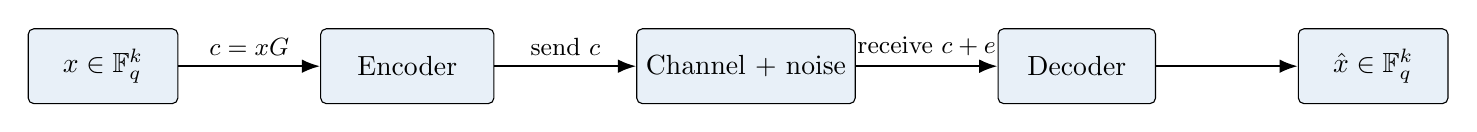
\begin{tikzpicture}[>=Latex, node distance=1.8cm]
  \node[draw, rounded corners=2pt, fill=softaccent, minimum width=1.9cm, minimum height=0.95cm] (data) {$x\in\F_q^k$};
  \node[draw, rounded corners=2pt, fill=softaccent, minimum width=2.2cm, minimum height=0.95cm, right=of data] (enc) {Encoder};
  \node[draw, rounded corners=2pt, fill=softaccent, minimum width=2.4cm, minimum height=0.95cm, right=of enc] (chan) {Channel + noise};
  \node[draw, rounded corners=2pt, fill=softaccent, minimum width=2.0cm, minimum height=0.95cm, right=of chan] (dec) {Decoder};
  \node[draw, rounded corners=2pt, fill=softaccent, minimum width=1.9cm, minimum height=0.95cm, right=of dec] (out) {$\hat x\in\F_q^k$};

  \draw[->, thick] (data) -- node[above, font=\small] {$c=xG$} (enc);
  \draw[->, thick] (enc) -- node[above, font=\small] {send $c$} (chan);
  \draw[->, thick] (chan) -- node[above, font=\small] {receive $c+e$} (dec);
  \draw[->, thick] (dec) -- (out);
\end{tikzpicture}
\end{center}

If
\[
G=[I_k\mid A],
\]
then the encoded word has the systematic form
\[
c=xG=(x_1,\dots,x_k,c_{k+1},\dots,c_n).
\]
This means that redundancy is appended after the information symbols.

\section{Generator and parity-check descriptions}

\subsection{Generator matrices}

\begin{definition}
Let $\code\subseteq \F_q^n$ be a linear $(n,k)$ code. A \emph{generator matrix} for $\code$ is a $k\times n$ matrix $G$ whose rows form a basis of $\code$. Equivalently,
\[
\code=\{xG:x\in\F_q^k\}.
\]
\end{definition}

Because the rows of $G$ span the code, every codeword is obtained as a linear combination of those basis vectors. The systematic form
\[
G=[I_k\mid A]
\]
is especially useful because the information symbols appear explicitly in the codeword.

\subsection{Parity-check matrices}

A linear code can also be described as the kernel of a matrix.

\begin{definition}
An \emph{parity-check matrix} for a linear $(n,k)$ code $\code\subseteq \F_q^n$ is an $(n-k)\times n$ matrix $H$ such that
\[
\code=\{v\in\F_q^n:Hv^T=0\}.
\]
\end{definition}

If the generator matrix is in systematic form $G=[I_k\mid A]$, then a compatible parity-check matrix is
\[
H=[-A^T\mid I_{n-k}].
\]
Indeed,
\[
G^T=
\begin{bmatrix}
I_k\\
A^T
\end{bmatrix},
\qquad
HG^T=[-A^T\mid I_{n-k}]
\begin{bmatrix}
I_k\\
A^T
\end{bmatrix}
=-A^T+A^T=0.
\]
So every codeword $c=xG$ satisfies
\[
Hc^T=H(xG)^T=HG^Tx^T=0.
\]
Since $H$ has rank $n-k$, its kernel has dimension $k$, which matches the dimension of $\code$.

\begin{proposition}
If $G=[I_k\mid A]$ generates an $(n,k)$ code $\code$, then $H=[-A^T\mid I_{n-k}]$ is a parity-check matrix for $\code$.
\end{proposition}

\begin{proof}
We already checked that every codeword lies in $\ker(H)$. Now $\dim \code=k$, while
\[
\dim \ker(H)=n-\operatorname{rank}(H)=n-(n-k)=k.
\]
A subspace of dimension $k$ contained in another subspace of dimension $k$ must be equal to it. Hence $\code=\ker(H)$.
\end{proof}

\section{The $(7,4)$ Hamming code}

The slide deck presents the binary Hamming code of length $7$ and dimension $4$. Over $\F_2$, the generator and parity-check matrices are
\[
G=
\begin{bmatrix}
1&0&0&0&0&1&1\\
0&1&0&0&1&0&1\\
0&0&1&0&1&1&0\\
0&0&0&1&1&1&1
\end{bmatrix},
\qquad
H=
\begin{bmatrix}
0&1&1&1&1&0&0\\
1&0&1&1&0&1&0\\
1&1&0&1&0&0&1
\end{bmatrix}.
\]
The matrix $G$ is in systematic form $[I_4\mid A]$, so the codeword corresponding to $x=(x_1,x_2,x_3,x_4)$ is
\[
xG=(x_1,x_2,x_3,x_4,\,x_2+x_3+x_4,\,x_1+x_3+x_4,\,x_1+x_2+x_4),
\]
where the additions are in $\F_2$.

The associated parity-check matrix satisfies $HG^T=0$, so the code may also be described as
\[
\code=\{v\in\F_2^7:Hv^T=0\}.
\]
This is the prototype example showing how generator and parity-check descriptions encode the same linear code.

\section{The dual code}

\subsection{Definition through a parity-check matrix}

Suppose $\code$ is an $(n,k)$ linear code over $\F_q$ with parity-check matrix $H$. The rows of $H$ are linearly independent and lie in $\F_q^n$. Since there are $n-k$ rows, they generate an $(n,n-k)$ code.

\begin{definition}
The \emph{dual code} of $\code$, denoted $\dual{\code}$, is the linear code generated by the rows of a parity-check matrix $H$ of $\code$.
\end{definition}

Thus if $\code$ has generator matrix $G$ and parity-check matrix $H$, then $\dual{\code}$ has generator matrix $H$.

\subsection{Definition through orthogonality}

The second definition uses the standard inner product on $\F_q^n$:
\[
x\cdot y^T=\sum_{i=1}^n x_i y_i.
\]

\begin{definition}
Let $\code\subseteq \F_q^n$ be a linear code. Its \emph{dual code} is
\[
\dual{\code}=\{v\in\F_q^n:c\cdot v^T=0\text{ for all }c\in\code\}.
\]
\end{definition}

This says that $\dual{\code}$ is the orthogonal complement of $\code$ with respect to the usual inner product.

\subsection{Equivalence of the two definitions}

\begin{proposition}
Let $G$ be a generator matrix for $\code$. Then
\[
\dual{\code}=\{v\in\F_q^n:Gv^T=0\}.
\]
In particular, the orthogonality definition and the parity-check-matrix definition of the dual code are equivalent.
\end{proposition}

\begin{proof}
Take $v\in\F_q^n$. Since every codeword has the form $c=xG$ for some $x\in\F_q^k$,
\[
c\cdot v^T=(xG)\cdot v^T=x(Gv^T).
\]
Therefore $c\cdot v^T=0$ for every $c\in\code$ if and only if $x(Gv^T)=0$ for every $x\in\F_q^k$. This happens precisely when
\[
Gv^T=0.
\]
So the orthogonal complement is exactly the kernel of $G$.
\end{proof}

This proposition has an immediate interpretation:
\begin{itemize}[leftmargin=1.4em]
    \item if $G$ generates $\code$, then $G$ is a parity-check matrix for $\dual{\code}$;
    \item if $H$ generates $\dual{\code}$, then $H$ is a parity-check matrix for $\code$.
\end{itemize}

\begin{theorem}
For every linear code $\code\subseteq \F_q^n$,
\[
(\dual{\code})^{\perp}=\code.
\]
\end{theorem}

\begin{proof}
If $G$ generates $\code$ and $H$ generates $\dual{\code}$, then $H$ is a parity-check matrix for $\code$, while $G$ is a parity-check matrix for $\dual{\code}$. Thus the code generated by $G$ is exactly the dual of the code generated by $H$. That is,
\[
(\dual{\code})^{\perp}=\code.
\]
One may also justify this by dimension counting: $\dim(\dual{\code})=n-k$, so $\dim((\dual{\code})^{\perp})=k$, and clearly $\code\subseteq (\dual{\code})^{\perp}$.
\end{proof}

\section{Repetition and single parity-check codes}

\subsection{Repetition code}

The $(n,1)$ repetition code over $\F_q$ is generated by
\[
G=[1\mid 1\ \cdots\ 1].
\]
Its codewords are
\[
(x_1)G=(x_1,x_1,\dots,x_1).
\]
So the only information symbol is repeated in every coordinate.

\subsection{Single parity-check code}

A systematic parity-check matrix for the repetition code over $\F_2$ is
\[
H=
\begin{bmatrix}
1&1&0&\cdots&0\\
1&0&1&\cdots&0\\
\vdots&\vdots&\vdots&\ddots&\vdots\\
1&0&0&\cdots&1
\end{bmatrix},
\]
which is exactly a generator matrix for the $(n,n-1)$ single parity-check code. Hence, over $\F_2$, the dual of the repetition code is the single parity-check code.

A vector $v=(v_1,\dots,v_n)$ belongs to the single parity-check code precisely when the coordinates add to zero:
\[
v_1+\cdots+v_n=0.
\]
Over $\F_2$, this means the Hamming weight of the vector is even.

\section{Self-orthogonal and self-dual codes}

\subsection{Self-orthogonal codes}

\begin{definition}
A linear code $\code$ is \emph{self-orthogonal} if
\[
\code\subseteq \dual{\code}.
\]
\end{definition}

The slides observe that the binary repetition code is self-orthogonal when $n$ is even.

\begin{proposition}
The $(n,1)$ repetition code over $\F_2$ is self-orthogonal if and only if $n$ is even.
\end{proposition}

\begin{proof}
The repetition code over $\F_2$ contains only two codewords:
\[
(0,\dots,0)\qquad \text{and}\qquad (1,\dots,1).
\]
For self-orthogonality, the vector $(1,\dots,1)$ must be orthogonal to itself. Its self-inner product is
\[
(1,\dots,1)\cdot(1,\dots,1)^T=1+\cdots+1=n\pmod 2.
\]
This equals $0$ in $\F_2$ exactly when $n$ is even.
\end{proof}

\subsection{Self-dual codes}

\begin{definition}
A linear code $\code$ is \emph{self-dual} if
\[
\code=\dual{\code}.
\]
\end{definition}

A self-dual code must have dimension $n/2$, so the ambient length must be even.

\section{The tetracode over $\F_3$}

The slides end with the classical $(4,2)$ tetracode over $\F_3$, generated by
\[
G=
\begin{bmatrix}
1&0&1&1\\
0&1&1&-1
\end{bmatrix}.
\]
Since we work over $\F_3$, the symbol $-1$ is the same as $2$.

\subsection{Parity-check calculation}

A parity-check matrix for this code is
\[
H=
\begin{bmatrix}
-1&-1&1&0\\
-1&1&0&1
\end{bmatrix}.
\]
By elementary row operations over $\F_3$, we can rewrite $H$ into the same systematic form as $G$:
\[
H
\sim
\begin{bmatrix}
-1&-1&1&0\\
0&2&-1&1
\end{bmatrix}
\sim
\begin{bmatrix}
-1&-1&1&0\\
0&1&1&2
\end{bmatrix}
\sim
\begin{bmatrix}
-1&0&2&2\\
0&1&1&2
\end{bmatrix}
\sim
\begin{bmatrix}
1&0&1&1\\
0&1&1&2
\end{bmatrix}=G.
\]
Thus $H$ and $G$ generate the same code, so the tetracode is self-dual.

\begin{proposition}
The tetracode generated by
\[
G=
\begin{bmatrix}
1&0&1&1\\
0&1&1&-1
\end{bmatrix}
\]
over $\F_3$ is self-dual.
\end{proposition}

\begin{proof}
A parity-check matrix for the code row-reduces to the same matrix $G$, so the dual code has the same generator matrix as the original code. Therefore $\dual{\code}=\code$.
\end{proof}

\subsection{Orthogonality calculation directly from the inner product}

A general codeword in the tetracode is
\[
c=(x_1,x_2,x_1+x_2,x_1-x_2), \qquad x_1,x_2\in\F_3.
\]
Take a vector $v=(v_1,v_2,v_3,v_4)\in\F_3^4$. For $v$ to lie in the dual code, we need
\[
v\cdot c^T=0
\quad\text{for all }x_1,x_2\in\F_3.
\]
Expanding gives
\[
v_1x_1+v_2x_2+v_3(x_1+x_2)+v_4(x_1-x_2)=0.
\]
Collecting coefficients of $x_1$ and $x_2$ yields the system
\[
v_1+v_3+v_4=0,
\qquad
v_2+v_3-v_4=0.
\]
Solving in $\F_3$ gives
\[
v_3=v_1+v_2,
\qquad
v_4=v_1-v_2.
\]
Hence every vector in the dual has the form
\[
(v_1,v_2,v_1+v_2,v_1-v_2),
\]
which is exactly the same parametrization as the original code. So again $\dual{\code}=\code$.

\section{Summary}

The slide deck can be summarized by the following dictionary:

\begin{center}
\renewcommand{\arraystretch}{1.35}
\begin{tabular}{>{\raggedright\arraybackslash}p{0.3\textwidth} >{\raggedright\arraybackslash}p{0.6\textwidth}}
\toprule
\textbf{Object} & \textbf{Description} \\
\midrule
Linear $(n,k)$ code $\code$ & A $k$-dimensional subspace of $\F_q^n$ \\
Generator matrix $G$ & Rows form a basis of $\code$; codewords are $xG$ \\
Parity-check matrix $H$ & $\code=\{v\in\F_q^n:Hv^T=0\}$ \\
Dual code $\dual{\code}$ & Orthogonal complement of $\code$ in $\F_q^n$ \\
Generator of $\dual{\code}$ & Any parity-check matrix of $\code$ \\
Parity-check of $\dual{\code}$ & Any generator matrix of $\code$ \\
Double dual & $(\dual{\code})^{\perp}=\code$ \\
Self-orthogonal code & $\code\subseteq \dual{\code}$ \\
Self-dual code & $\code=\dual{\code}$ \\
\bottomrule
\end{tabular}
\end{center}

\section*{Exercises for review}
\addcontentsline{toc}{section}{Exercises for review}

\begin{exercise}
Verify directly that the Hamming matrices in Section 3 satisfy $HG^T=0$ over $\F_2$.
\end{exercise}

\begin{exercise}
Show that the dimension of $\dual{\code}$ is $n-k$ when $\dim \code=k$.
\end{exercise}

\begin{exercise}
Let $\code$ be the binary repetition code of length $n$. Describe $\dual{\code}$ explicitly and verify that it is the single parity-check code.
\end{exercise}

\begin{exercise}
For the tetracode, list all nine codewords of the code by allowing $(x_1,x_2)$ to run through $\F_3^2$.
\end{exercise}

\end{document}
